% \section{Auswertung}
% \label{sec:Auswertung}

\section{Auswertung}
\subsection{Fouriersynthese}
\begin{figure}
    \begin{subfigure}{0.5\textwidth}
        \centering
        \includegraphics[width=\textwidth]{assets/20231114_125400.jpg}
        \caption{Rechteckschwingung}
    \end{subfigure}
    \begin{subfigure}{0.5\textwidth}
        \centering
        \includegraphics[width=\textwidth]{assets/20231114_130609.jpg}
        \caption{Dreieckschwingung}
    \end{subfigure}
    \begin{subfigure}{0.5\textwidth}
        \centering
        \includegraphics[width=\textwidth]{assets/20231114_132155.jpg}
        \caption{Sägezahnschwingung}
    \end{subfigure}
    \caption{Mit dem Oszilloskop aufgezeichnete Schwingungsbilder}
    \label{fig:oszi}
\end{figure}

In Abbildung \ref{fig:oszi} sind die aufgezeichneten Schwingungsbilder für die
drei eingestellten Schwingungen dargestellt. Es zeigt sich, dass alle drei in
guter Übereinstimmung mit den in der Vorbereitung vorhergesagten Kurven stehen.

\subsection{Fourieranalyse}
\subsubsection{Rechteckschwingung}
\begin{table}[h]
    \centering
    \caption{Aufgenommene Messwerte zur Rechteckspannung}
    \label{tab:rechteck_messwerte}
    \begin{tabular}{ S S S S }
        \toprule
        { $\text{Oberschwingung} \: n $ } & { $ \nu \: / \: \si{kHz} $} & {$ \text{Amplitude} \: / \: \si{dB} $} & {$ \text{Amplitude}\: U \: / \: \si{V} $} \\
        \midrule
        1                                 & 100                         & 39.0                                   & 89.12                                     \\
        3                                 & 300                         & 29.4                                   & 29.51                                     \\
        5                                 & 500                         & 25.0                                   & 17.78                                     \\
        7                                 & 700                         & 22.2                                   & 12.88                                     \\
        9                                 & 900                         & 20.6                                   & 10.71                                     \\
        11                                & 1100                        & 19.0                                   & 8.91                                      \\
        13                                & 1300                        & 17.8                                   & 7.76                                      \\
        15                                & 1500                        & 16.6                                   & 6.76                                      \\
        17                                & 1700                        & 16.2                                   & 6.45                                      \\
        19                                & 1900                        & 15.4                                   & 5.88                                      \\
    \end{tabular}
\end{table}
In Tabelle \ref{tab:rechteck_messwerte} sind die vom Oszilloskop abgelesenen Positionen und Höhen der Peaks der Rechteckschwingung aufgetragen. Wie in der Vorbereitung vorhergesagt, lassen sich keine peaks für gerade $n$ messen.
Zur Überprüfung der $n$-Abhängigkeit ist in Abbildung \ref{fig:rechteck_fit} die Höhe der Peaks einmal direkt gegen die Frequenz und einmal gegen $\frac{1}{n}$ aufgetragen. Bei letzterem ist zu sehen, dass alle Messwerte näherungsweise auf einer Geraden liegen. Der Fit ist eine Gerade der Form
\begin{equation*}
    y = ax + b
\end{equation*}
mit den Parametern
\begin{align*}
    a = \SI{88.011 \pm 0.520}{V}
    b = \SI{0.805 \pm 0.181}{V} .
\end{align*}
\begin{figure}[h]
    \begin{subfigure}{0.5\textwidth}
        \centering
        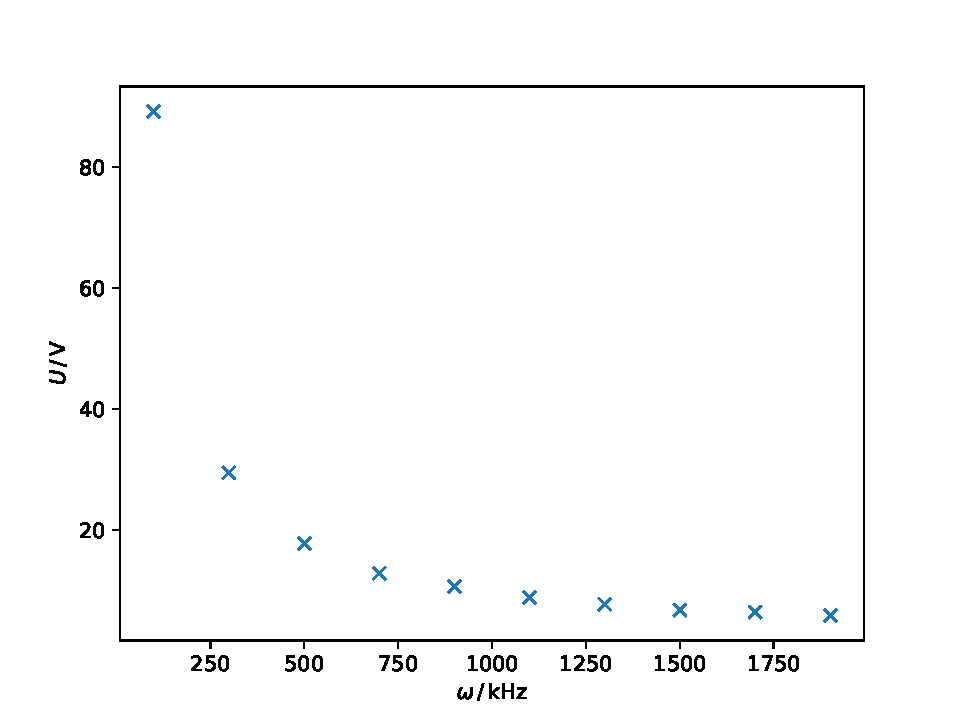
\includegraphics[width=\textwidth]{assets/rechteck_messung.pdf}
    \end{subfigure}
    \begin{subfigure}{0.5\textwidth}
        \centering
        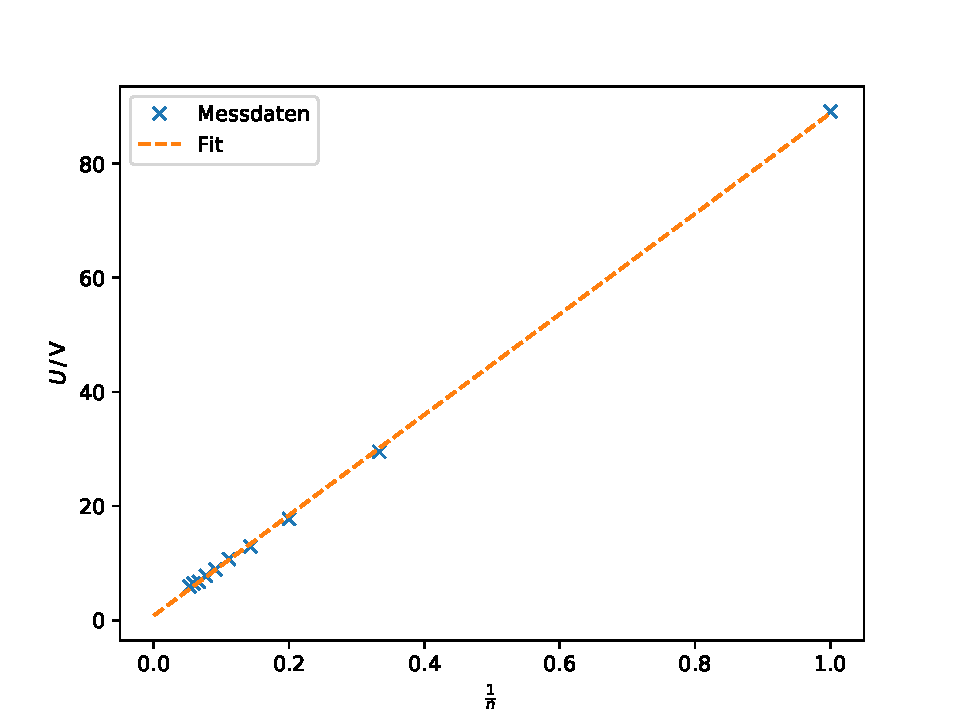
\includegraphics[width=\textwidth]{assets/rechteck_fit.pdf}
    \end{subfigure}
    \caption{Messdaten für die Rechteckschwingung}
    \label{fig:rechteck_fit}
\end{figure}

\subsubsection{Dreieckschwingung}
\begin{table}[h]
    \centering
    \caption{Aufgenommene Messwerte zur Dreieckspannung}
    \label{tab:dreieck_messwerte}
    \begin{tabular}{ S S S S }
        \toprule
        { $\text{Oberschwingung} \: n $ } & { $ \nu \: / \: \si{kHz} $} & {$ \text{Amplitude} \: / \: \si{dB} $} & {$ \text{Amplitude}\: U \: / \: \si{V} $} \\
        \midrule
        1                                 & 100                         & 35.00                                  & 56.23                                     \\
        3                                 & 300                         & 16.20                                  & 6.46                                      \\
        5                                 & 500                         & 7.01                                   & 2.241                                     \\
        7                                 & 700                         & 1.81                                   & 1.23                                      \\
        9                                 & 900                         & -2.99                                  & 0.71                                      \\
        11                                & 1100                        & -6.59                                  & 0.47                                      \\
        13                                & 1300                        & -8.59                                  & 0.37                                      \\
    \end{tabular}
\end{table}
In Tabelle \ref{tab:dreieck_messwerte} sind wieder die abgelesenen Positionen und Höhen der Peaks der Dreieckschwingung aufgetragen. Wie bei der Rechteckschwingung, lassen sich keine Peaks für gerade $n$ messen. Wie zuvor sind in Abb. \ref{fig:dreieck_fit} die Höhen der Peaks einmal gegen die Frequenzen und diesmal gegen $\frac{1}{n^2}$ aufgetragen.
Letztere Abbildung zeigt wieder, dass die Messwerte näherungsweise auf einer Geraden liegen. Die Ausgleichsgerade hat die Parameter
\begin{align*}
    a = \SI{56.193 \pm 0.092}{V}
    b = \SI{0.056 \pm 0.035}{V} .
\end{align*}
\begin{figure}[h]
    \begin{subfigure}{0.5\textwidth}
        \centering
        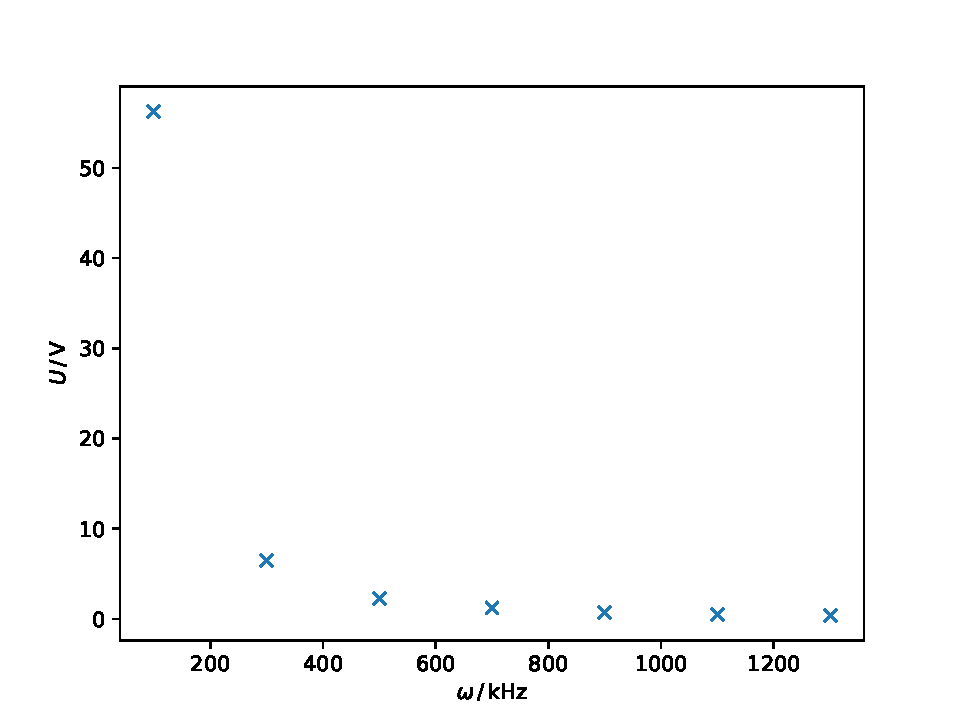
\includegraphics[width=\textwidth]{assets/dreieck_messung.pdf}
    \end{subfigure}
    \begin{subfigure}{0.5\textwidth}
        \centering
        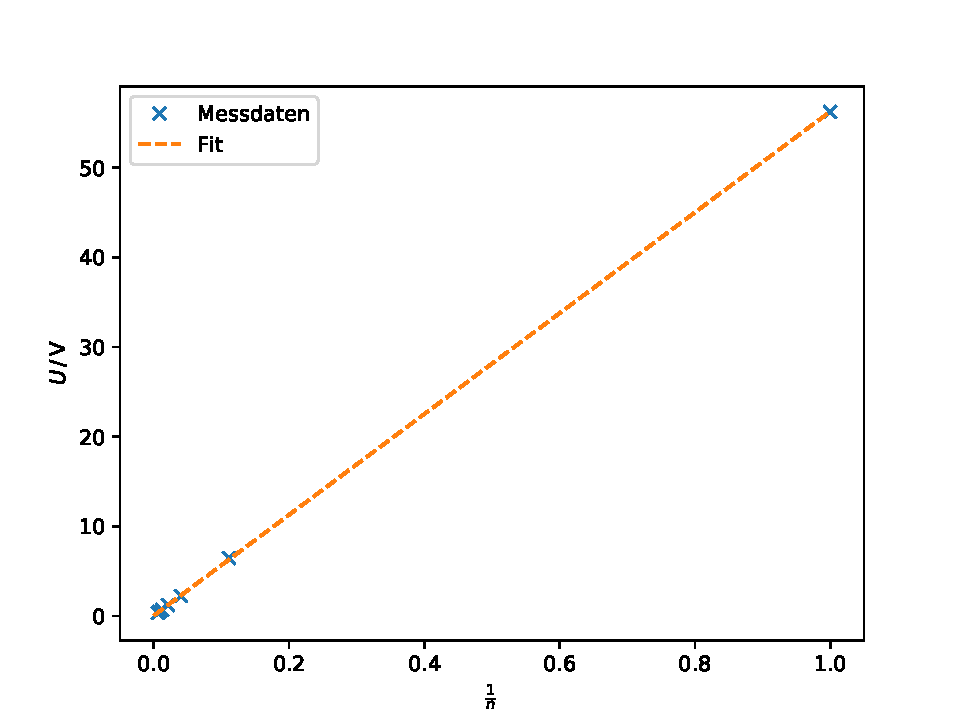
\includegraphics[width=\textwidth]{assets/dreieck_fit.pdf}
    \end{subfigure}
    \caption{Messdaten für die Dreieckschwingung}
    \label{fig:dreieck_fit}
\end{figure}
\subsubsection{Sägezahnschwingung}
\begin{table}[h]
    \centering
    \caption{Aufgenommene Messwerte zur Sägezahnspannung}
    \label{tab:zahn_messwerte}
    \begin{tabular}{ S S S S }
        \toprule
        { $\text{Oberschwingung}\: n $ } & { $ \nu \: / \: \si{kHz} $} & {$ \text{Amplitude} \: / \: \si{dB} $} & {$ \text{Amplitude}\: U \: / \: \si{V} $} \\
        \midrule
        1                                & 100                         & 32.8                                   & 43.65                                     \\
        2                                & 205                         & 27.0                                   & 22.38                                     \\
        3                                & 305                         & 22.6                                   & 13.49                                     \\
        4                                & 405                         & 21.4                                   & 11.75                                     \\
        5                                & 505                         & 19.8                                   & 9.77                                      \\
        6                                & 605                         & 18.2                                   & 8.13                                      \\
        7                                & 705                         & 17.4                                   & 7.41                                      \\
        8                                & 810                         & 16.6                                   & 6.76                                      \\
        9                                & 910                         & 15.8                                   & 6.16                                      \\
        10                               & 1010                        & 15.4                                   & 5.89                                      \\
    \end{tabular}
\end{table}
Tabelle \ref{tab:zahn_messwerte} zeigt wieder die Positionen und Höhen der Peaks. Anders als bei den vorherigen Schwingungen sind hier auch Peaks für gerade $n$ messbar. In Abb. \ref{fig:zahn_fit} sind die Werte gegen die Frequenzen und gegen $\frac{1}{n}$ aufgetragen. Es lässt sich, wie vorhergesagt, ein linearer Zusammenhang zwischen der Höhe der Peaks und $\frac{1}{n}$ feststellen. Die Ausgleichsgerade hat die Parameter
\begin{align*}
    a = \SI{42.068 \pm 0.812}{V}
    b = \SI{1.219 \pm 0.320}{V} .
\end{align*}
\begin{figure}[h]
    \begin{subfigure}{0.5\textwidth}
        \centering
        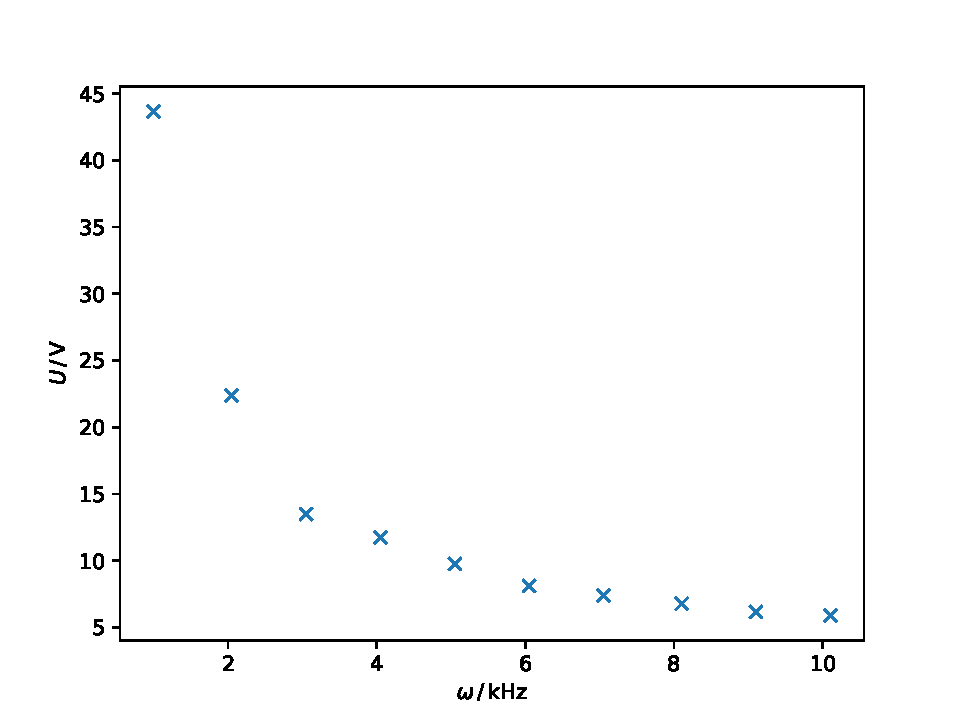
\includegraphics[width=\textwidth]{assets/zahn_messung.pdf}
    \end{subfigure}
    \begin{subfigure}{0.5\textwidth}
        \centering
        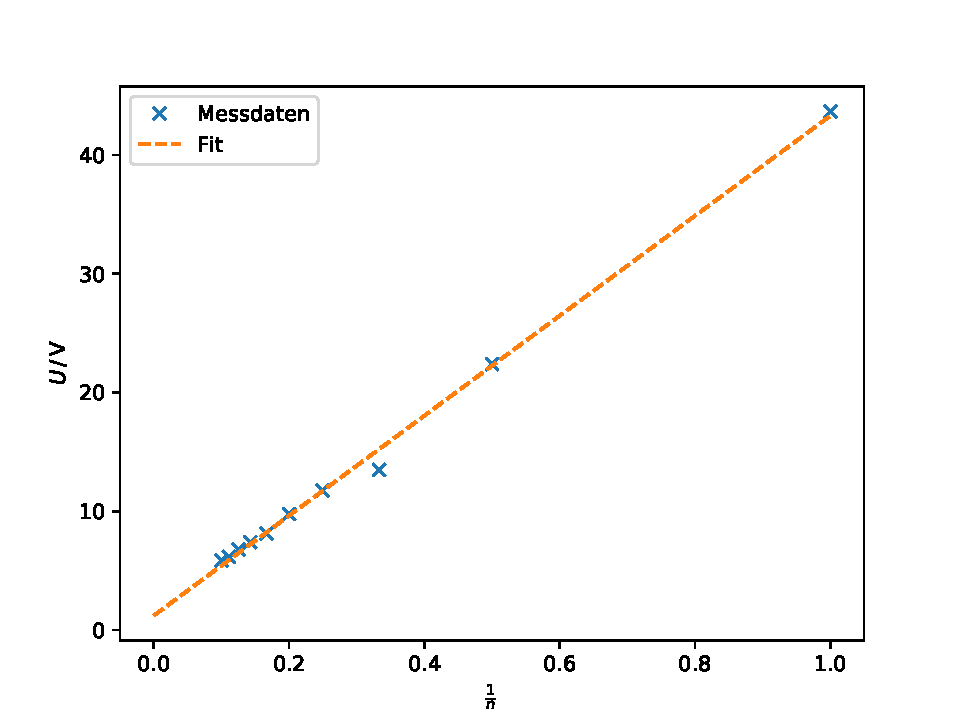
\includegraphics[width=\textwidth]{assets/zahn_fit.pdf}
    \end{subfigure}
    \caption{Messdaten für die Sägezahnschwingung}
    \label{fig:zahn_fit}
\end{figure}
%   \caption{Fourier-Annäherung einer Sägezahnschwingung für $n=9$}
%   \label{fig:vorbereitung_sägezahn}
% \end{figure}
